\documentclass[a4paper,leqno]{article}
\usepackage[utf8]{inputenc}
\usepackage{lmodern}
\usepackage{microtype}
\usepackage[inline]{enumitem}

\usepackage{siunitx}
\usepackage{multirow}
\usepackage{subcaption}

\usepackage[english]{babel}
\usepackage[autostyle, english=british]{csquotes}
\MakeOuterQuote{"}

\usepackage{commath}
\usepackage{amsmath}
\usepackage{amsthm}
\usepackage{amssymb}
\usepackage{mathtools}

\usepackage{pgfplots}
\pgfplotsset{compat=1.11}
\usepgfplotslibrary{fillbetween}
\usetikzlibrary{patterns}

\usepackage{hyperref}

\usepackage[margin=1in]{geometry}
\usepackage{changepage}
\usepackage{titlesec}
\titleformat{\section}{\normalfont\Large\bfseries\centering}{Section~\thesection:}{1em}{}

\def\signed #1{{\leavevmode\unskip\nobreak\hfil\penalty50\hskip2em
  \hbox{}\nobreak\hfil(#1)%
  \parfillskip=0pt \finalhyphendemerits=0 \endgraf}}
\newsavebox\mybox
\newenvironment{aquote}[1]
  {\savebox\mybox{#1}\begin{quote}}
  {\signed{\usebox\mybox}\end{quote}}

% Augmented matrices.
\makeatletter
\renewcommand*\env@matrix[1][*\c@MaxMatrixCols c]{%
  \hskip -\arraycolsep
  \let\@ifnextchar\new@ifnextchar
  \array{#1}}
\makeatother

%--------grstep
% For denoting a Gauss' reduction step.
% Use as: \grstep{\rho_1+\rho_3} or \grstep[2\rho_5 \\ 3\rho_6]{\rho_1+\rho_3}
\newcommand{\grstep}[2][\relax]{%
   \ensuremath{\mathrel{
       {\mathop{\longrightarrow}\limits^{#2\mathstrut}_{
                                     \begin{subarray}{l} #1 \end{subarray}}}}}}
\newcommand{\swap}{\leftrightarrow}


\swapnumbers
\numberwithin{equation}{section}
\newtheorem{thm}[equation]{Theorem}
\newtheorem{lem}[equation]{Lemma}
\newtheorem{cor}[equation]{Corollary}
\newtheorem{prp}[equation]{Proposition}
\theoremstyle{definition}
\newtheorem{defn}[equation]{Definition}
\newtheorem{ex}[equation]{Example}
\newtheorem{exercise}[equation]{Exercise}
\newtheorem{alg}[equation]{Algorithm}
\newtheorem{axiom}[equation]{Axiom}
\theoremstyle{remark}
\newtheorem{rem}[equation]{Remark}

\newcommand{\df}[1]{\textbf{#1}}
\newcommand{\T}{\mathrm{T}}
\newcommand{\F}{\mathrm{F}}
\newcommand{\IndSet}{\mathbf{I}}
\DeclareMathOperator{\cis}{cis}

\title{Level Three Conic Sections}
\author{Alex Elzenaar}
\date{\today}

\begin{document}
\maketitle
\tableofcontents
\section*{Preface}
The conic sections are the simplest curves in the plane which are not simply straight lines. However, most secondary school treatments of the subject
tend to present a set of vaguely connected case-by-case results, rather than any kind of coherent story. These notes are my attempt to avoid this.

\subsection*{Prerequisites}
These notes have perhaps the most `formal' prerequisites out of all my Y13 notes. I will assume results from trigonometry, linear systems, calculus, and
even algebra. However, this does not mean that the full power of these subjects are used. The most important prerequisites are actually Y11 and Y12
geometry because there are a number of results from there about triangles, circles, lines, and so forth that will be used here. My Y13 notes on trigonometry
revise a number of these results, and so the reader is directed there initially.

\begin{center}
  \includegraphics[width=0.4\textwidth]{conics}
\end{center}

\titleformat{\section}{\clearpage\titlerule[0.8pt]\vspace{0.5ex}\normalfont\Large\bfseries\centering}{Section~\thesection:}{1em}{}[{\titlerule[0.8pt]}]
\let\oldsection\section
\renewcommand\section{\clearpage\oldsection}
\section{Quadratic Equations (Again)}
\begin{center}
  \emph{You know, for a mathematician, he did not have enough imagination. But he has become a poet and now he is fine.} --- Hilbert (on an ex-student)
\end{center}
We will study in this topic precisely equations of the form
\begin{equation}\label{eqn:prototype}
  ax^2 + 2hxy + by^2 + 2gx + 2fy + c = 0.
\end{equation}
This class of equations is the class of \df{quadratic equations} (in two variables). Note that, without loss
of generality, we can assume $ c = 1 $ (otherwise, we just divide through by $ c $).

The set of all points $ (x,y) $ satisfying a quadratic equation is called a \df{curve of the second degree}.

Our first theorem is a generalisation of the statement from algebra that every quadratic equation in one variable
(i.e. every equation $ x^2 + px + q = 0 $) has precisely two solutions (if you count correctly).
\begin{thm}\label{thm:funthmquad}
  Every line meets a curve of the second degree in precisely two points.
\end{thm}

This theorem is very nice, but (like the proof for quadratics in one variable) we do have to make a trade:
we have to take our coordinate system to be over the complex numbers. Thus, for the remainder of these notes,
we will assume implicitly that rather than living in the real plane $ \mathbb{R}^2 $ we are in fact living
in the complex plane $ \mathbb{C}^2 $. In some sense, then, we are doing geometry in four dimensions. On the
other hand, in many places we will only be interested in real coordinates. For example, the graph of a four-dimensional
object is a little tricky to draw if we only have three dimensions available!

Our first proof attempt looks all right, and indeed it is almost correct;

\begin{proof}[Proof attempt]
  Let $ ax + by = 1 $ be our line. At least one of $ a $ or $ b $ is non-zero; assume that $ a $ is
  non-zero (but essentially the same proof will work if $ a = 0 $ but $ b $ is non-zero). Then we
  can substitute $ x = \frac{1 - by}{a} $ into our curve of the second degree to obtain a quadratic
  equation in the variable $ y $; by the fundamental theorem of algebra, this equation has two solutions;
  and each of these corresponds with a point of intersection.
\end{proof}

The problem with this proof is illustrated by the following example:-
\begin{ex}
  Consider the quadratic $ xy + y + x^2 = 1 $. This describes a perfectly good curve in two dimensions, graphed here.
  \begin{center}
    \fbox{\begin{tikzpicture}
      \begin{axis}[
        axis lines = center,
        xlabel = $ x $,
        ylabel = $ y $
      ]
        \addplot[domain = -5:5, color = red] {1-x};
        \draw[color = red] ({axis cs:-1,0}|-{rel axis cs:0,0}) -- ({axis cs:-1,0}|-{rel axis cs:0,1});
      \end{axis}
    \end{tikzpicture}}
  \end{center}
  If we intersect this curve with the line $ y = 2 - x $, then we obtain a linear equation $ x + 2 = 0 $ instead of a quadratic
  equation --- and so even counting multiplicities and moving up to $ \mathbb{C} $, we only have one solution.
\end{ex}

The reader might be tempted to discount this example as uninteresting, because it's simply the intersection of a pair of two lines
with a third line and thus isn't really a problem that affects our programme of studying curves of the second degree.

The next example, though, is both more fundamental and more worrying.
\begin{ex}
  If we intersect the parabola $ x^2 = y $ with the line $ x = 0 $, we obtain a single point of intersection, even
  up to multiplicity.
\end{ex}

Does this mean that we have to abandon the beautiful intersection theorem?

It turns out that, like how we expanded our number system to make the fundamental theorem of algebra work
nicely, we can expand our plane $ \mathbb{C}^2 $ further to make our intersection theorem work.

We will not make this precise, but the method we will use is some kind of limiting process; the result, and the
system we will work in from now on, is the projective plane over $ \mathbb{C} $. Let us see how we climb to it.

\subsection{Euclidean Geometry}
It turns out that in order to approach some kind of resolution, we need to mention the elephant in the room: the
foundation of all the geometry which we have been doing thus far in our mathematical lives. (This might seem at first
glance completely unrelated to the algebraic problem we're trying to solve, but bear with me.)

In ancient Greece, in about 300~BCE, Euclid of Alexandria (in Egypt) wrote his book \emph{Elements}, one of the most
influential mathematical texts of all time. In it, he set down the set of basic results which can be proved true
about circles and lines on a plane: while modern geometry has gone much further than Euclid (in considering geometry in more than
two dimensions, and on surfaces much more complicated than the plane), the basic results which are taught in any
introductory geometry course are usually treated in the Elements.

Euclid was influential because he was the first author (or, more likely, the first author whose work survives) to
attempt to rigorously prove all his results based on a set of `universal truths': a set of simple statements (called
\df{axioms}) whose truth is self-evident. In some sense, the goal of mathematics is to deduce the behaviour of the
most complicated systems possible from the simplest axioms possible.\footnote{The axiom system which most of modern
mathematics is done within is called ZFC (Zermelo-Fraenkel with Choice, named after two mathematicians working on the
area in the early 1900s).} Euclid's axioms were as follows:
\begin{enumerate}
  \item A straight line segment can be drawn joining any two points.
  \item Any straight line segment can be extended indefinitely in a straight line.
  \item Given any straight line segment, a circle can be drawn having the segment as radius and one endpoint as center.
  \item All right angles are congruent.
  \item Given any straight line and a point not on it, there exists one and only one straight line which passes through
        that point and never intersects the first line, no matter how far they are extended.
\end{enumerate}
Putting aside the fact that these axioms are in fact insufficient for the purpose of constructing plane geometry, it is
clear that the fifth axiom is both far less elegant than the others and far more complicated. Indeed, Euclid himself avoided
using it in his proofs except where necessary (he avoids it completely for the first 28 propositions, for example) and for
many years mathematicians believed that it was in fact a theorem: that it could be proved from the previous four axioms.

It turns out that this is false: there exist geometries for which the fifth axiom is false (for example, on a sphere).

\subsection{Projective Geometry}
The mathematical world which we are interested in is known as \df{projective geometry} (the name will only make sense towards
the end of these notes). We obtain this geometry by replacing the final axiom with the following axiom:
\begin{axiom}[Elliptic incidence property]
  Any two distinct lines in a projective geometry meet at exactly one point.
\end{axiom}
This is clearly not true in usual Euclidean geometry. On the other hand, we didn't let this kind of thing stop us in the
past: the number $ i $ is absolutely useless for counting sheep, for example, but that doesn't stop the complex numbers from
being an interesting (and useful) mathematical space.

The complex numbers became much clearer once we stopped thinking about numbers as a line and started drawing them as a plane. There
is an analogous simple way to construct and think about a projective plane by extending the Euclidean plane (and then extending our
setting, the complex plane, will be done in the same way).

When we think about it, we find that the only reason that Euclidean geometry doesn't satisfy this axiom is that parallel lines exist.
We will therefore \emph{define them not to exist}!

More precisely, given every set of parallel lines with slope $ m $, we will take our plane and add on a new point $ \infty_m $ called
a \emph{point at infinity}, and then define this new point to be on all the lines with slope $ m $. Thus, these parallel lines now
intersect at exactly one point (the point at infinity related to their slope) and all other lines intersect in exactly one point (the
same place they did before).

\begin{center}
  \includegraphics[width=0.5\textwidth]{vanishingpoint}
\end{center}

This can be made to make some sense physically, and indeed the first place which projective geometry appeared was when Renaissance artists
like Leonardo da Vinci began to experiment with perspective drawing --- if you look down two parallel lines in real life, like those in the
image above,\footnote{© Vespertunes / Wikimedia Commons / ``Vanishing Point of Railway''. \url{https://commons.wikimedia.org/wiki/File:Vanishing_Point_of_Railway.jpg}}
they appear to meet at the horizon, and lines going in the same direction away from you (i.e. lines with the same slope) meet
at the same point. We call the line joining all the points at infinity (in this physical case, the horizon) the \df{line at infinity}.

Going back to our problem of curves of the second degree, let us consider our second example: $ x^2 = y $ only intersects the line $ x = 0 $
at one point.

\begin{center}
  \fbox{\begin{tikzpicture}
    \begin{axis}[
      axis lines = center,
      xlabel = $ x $,
      ylabel = $ y $, ymin=-2
    ]
      \addplot[domain = -5:5, color = red] {x^2};
      \draw[color = blue] ({axis cs:0,0}|-{rel axis cs:0,0}) -- ({axis cs:0,0}|-{rel axis cs:0,1});
    \end{axis}
  \end{tikzpicture}}
\end{center}

But notice, as $ x \to \pm \infty $ the curve $ x^2 $ tends towards being vertical! More precisely, we have
that $ \lim_{x \to \infty} \od{}{x} x^2 = \infty $; thus, the parabola is \df{eventually parallel} to the
vertical line, and so the two intersect for a second time at the point at infinity $ \infty_\infty $.

This is even more blatant in our first example: we had the following curve (and again, the blue line is the
line we intersect with our second degree curve):

\begin{center}
  \fbox{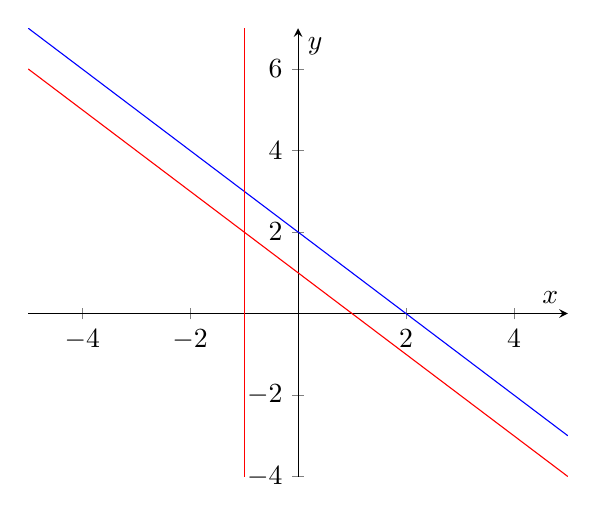
\begin{tikzpicture}
    \begin{axis}[
      axis lines = center,
      xlabel = $ x $,
      ylabel = $ y $
    ]
      \addplot[domain = -5:5, color = red] {1-x};
      \addplot[domain = -5:5, color = blue] {2-x};
      \draw[color = red] ({axis cs:-1,0}|-{rel axis cs:0,0}) -- ({axis cs:-1,0}|-{rel axis cs:0,1});
    \end{axis}
  \end{tikzpicture}}
\end{center}

In this case, the curve is not only \emph{eventually} parallel, but in fact it is \emph{actually} parallel!

The picture to keep in mind, for conic sections at least, is the following.

\begin{center}
  \includegraphics[width=0.3\textwidth]{infiniteparabola}
\end{center}

Note that this picture does not actually reflect what is \emph{really} going on when we graph second degree
equations in the plane --- it's a diagrammatic representation of the fact that we've made a fundamental extension
to our system of geometry (and to our system of algebra, but this isn't visible on a real graph).

Philosophically, all we've done is decided what property we want our algebro-geometric system to have (that
curves of the second degree intersect any line at exactly two places, unless it's tangent to the line) and then
invented a geometry in which this property is true. It turns out that this geometry has a lot of other beautiful
properties, most of which we don't have time to look at --- but at this stage, it's completely synthetic. We simply
arbitrarily added a bunch of points (and we're honestly lucky we didn't get any contradictions). In fact, eventually
we will see that there is an incredibly natural way to construct a projective plane without having to worry about
sticking in a bunch more points and cooking it ourselves. For now, we will content ourselves with proving
our motivational theorem.

\subsection{Proof of Theorem \ref{thm:funthmquad}}

Let $ y = mx + n $ be our line. Then we can substitute $ y $ into our curve of the second degree to obtain an equation
in the variable $ x $ which is either of degree 1 or degree 2. (If necessary, let $ m $ be infinite.)

\paragraph{Case I.} If the equation is of degree two, then by the fundamental theorem of algebra it
has two solutions; and each of these corresponds with a point of intersection.

\paragraph{Case II.} We will be done if we can show the following: if a line $ y = mx + n $ intersects
some quadratic equation $ ax^2 + 2hxy + by^2 + 2gx + 2fy + c = 0 $ in exactly one point (i.e. in such a
way as to produce a linear equation in $ x $ rather than a quadratic) then
\begin{equation}
  \lim_{x \to \infty} y'(x) = m
\end{equation}

Step 1. We will find the condition on the coefficients of our quadratic for $ x^2 $ to vanish upon substitution.
So let us substitute $ y = mx + c $ into our quadratic; we obtain
\begin{displaymath}
  ax^2 + 2hx(mx + c) + b(mx + c)^2 + 2gx + 2f(mx + c) + c = 0
\end{displaymath}

Expanding, and setting the coefficient of the $ x^2 $ term to zero, we find that
\begin{displaymath}
  a + 2mh + bm^2 = 0.
\end{displaymath}

Step 2. We will find the derivative $ y'(x) $; this is a simple exercise in implicit differentiation and we get that
\begin{displaymath}
  \od{y}{x} = -\frac{ax + hy + g}{hx + by + f}.
\end{displaymath}
Substituting our condition on the coefficients, we have
\begin{displaymath}
  \od{y}{x} = -\frac{-2mhx - bm^2x + hy + g}{hx + by + f}.
\end{displaymath}

Step 3. Taking limits of both sides, we have
\begin{displaymath}
  \lim_{x \to \infty} \od{y}{x} = \lim_{x \to \infty} -\frac{-2mhx - bm^2x + hy + g}{hx + by + f}.
\end{displaymath}

It is not immediately obvious how we should deal with this right-hand side, because $ y $ also depends
on $ x $. Looking at the equation for the quadratic, we note that as $ x \to \infty $, we must have $ y \to \pm\infty $ ---
otherwise the right hand side couldn't stay at zero. Therefore, both the top and the bottom of the fraction under our
limit go to infinity; we can apply the following theorem (which we will not prove here):

\begin{thm}[l'Hopital's Rule]
  If $ \lim_{x \to \infty} f(x) = \infty $ and $ \lim_{x \to \infty} g(x) = \infty $, and if $ \lim_{x\to\infty} f'(x)/g'(x) = l $,
  then $ \lim_{x\to\infty} f(x)/g(x) = l $.\footnote{Proof: see Spivak, chapter 11, theorem 9 and exercises 36-38.\qed}
\end{thm}

Let $ \lim_{x \to \infty} \od{y}{x} = L $. Then we have
\begin{displaymath}
  L = \lim_{x \to \infty} -\frac{-2mhx - bm^2x + hy + g}{hx + by + f} = \lim_{x \to \infty} -\frac{-2mh - bm^2 + h\od{y}{x}}{h + b\od{y}{x}}
                                                                      = -\frac{-2mh - bm^2 + hL}{h + bL}
\end{displaymath}
and $ 0 = bL^2 + 2hL - 2mh - bm^2 $, so
\begin{displaymath}
  L = \frac{-2h + \sqrt{4h^2 + 4b(2mh + bm^2)}}{2b} = \frac{-2h + 2\sqrt{h^2 + 2bmh + bm^2}}{2b}
                                                    = \frac{-2h + 2(h + bm)}{2b} = m
\end{displaymath}
Thus we have shown that if the derivative $ \od{y}{x} $ tends to any value, it must tend to $ m $.

Suppose $ \od{y}{x} $ does not tend to a finite number. If $ \od{y}{x} $ goes to infinity, then in
particular it intersects every non-vertical line at two points (draw a picture), so if the line intersects
at precisely one point then it is vertical; thus if $ m = \infty $ then $ \od{y}{x} \to \infty $. On
the other hand, $ \od{y}{x} $ is either eventually positive or eventually negative (just by inspecting
the expression for it above), so it either tends to infinity or to some finite limit.
\qed

\section{Classifying Curves of the Second Degree}
Now that we know the correct system to frame our discussion in, we will begin to carry out our first major programme: the
classification of all the different kinds of conic sections. Our goal is to determine, by looking at a quadratic equation,
what the form of curve on the real plane it describes.

\subsection{Polar Form}
Recall that the plane can be given coordinates in two very natural ways: rectangular coordinates, and polar coordinates.

\section{Isometries}
I claim that the graph of every quadratic equation like \ref{eqn:prototype} is just a translated and
rotated version of the graph of an equation with the form
\begin{equation}
  px^2 + qy^2 = 1.
\end{equation}

In order to show this, we need to study the effect of rotations and translations on coordinate systems. We
begin with rotations because it turns out that rotating before translating is easier for our purposes.

Let $ \rho = \cis \theta $ be a complex number such that $ \abs{\rho} = 1 $. If $ z = x + yi $ is a point on the complex plane,
then $ \rho $ acts by multiplication on $ z $ to rotate it around the origin by an angle $ \theta $; we can then calculate
the resulting rectangular coordinates of $ \rho z $ to see how a rotation affects our normal coordinate system.
\begin{align*}
  z &= \abs{z} \cis(\tan^{-1} x/y)\\
  \rho z &= \abs{z} \cis(\tan^{-1} x/y + \theta)\\
         &= \abs{z} \left[\cos(\tan^{-1} x/y + \theta) + i\sin(\tan^{-1} x/y + \theta)\right].
\end{align*}

Using trig identities, we calculate
\begin{align*}
  \cos(\tan^{-1} x/y + \theta) = \cos(\tan^{-1} x/y) \cos \theta - \sin(\tan^{-1} x/y) \sin \theta\\
                               = \frac{x}{\sqrt{x^2 + y^2}} \cos \theta - \frac{y}{\sqrt{x^2 + y^2}} \sin \theta\\
  \sin(\tan^{-1} x/y + \theta) = \sin(\tan^{-1} x/y) \cos \theta + \cos(\tan^{-1} x/y) \sin \theta\\
                               = \frac{y}{\sqrt{x^2 + y^2}} \cos \theta + \frac{x}{\sqrt{x^2 + y^2}} \sin \theta
\end{align*}
and so
\begin{align*}
  \rho z &= \abs{z} \left[\cos(\tan^{-1} x/y + \theta) + i\sin(\tan^{-1} x/y + \theta)\right]\\
         &= (x \cos \theta - y \sin \theta) + i(y \cos \theta + x \sin \theta).
\end{align*}

In other words, if the point $ (x,y) $ is rotated about the origin by an angle $ \theta $, then
\begin{equation}
  (x,y) \xmapsto{\rho} (x \cos \theta - y \sin \theta,y \cos \theta + x \sin \theta).
\end{equation}

Considering $ ax^2 + bx + cxy + dy + ey^2 $, then, we want to rotate $ (x,y) $ by some $ \theta $ so that some terms vanish. Doing
a long computation, we find that
\begin{align*}
  ax^2 + bx + cxy + dx + ey^2 &= a(x \cos \theta - y \sin \theta)^2 + b(x \cos \theta - y \sin \theta)\\
                              &  \qquad + c(x \cos \theta - y \sin \theta)(y \cos \theta + x \sin \theta)\\
                              &  \qquad + d(y \cos \theta + x \sin \theta) + e(y \cos \theta + x \sin \theta)^2\\
                              &= ax^2 \cos^2 \theta - 2axy \cos\theta\sin\theta + ay^2 \sin^2\theta + bx\cos\theta - by\sin\theta\\
                              &  \qquad + cxy \cos^2 \theta + cx^2 \sin \theta\cos\theta - cy^2 \sin\theta\cos\theta - cxy \sin^2\theta\\
                              &  \qquad + dy\cos\theta + dx\sin\theta + ey^2\cos^2\theta + 2exy\cos\theta\sin\theta + ex^2\sin^2\theta\\
                              &= x^2(a\cos^2 \theta + \frac{c}{2}\sin 2\theta + e\sin^2 \theta) + x(b \cos \theta + d\sin \theta)\\
                              &  \qquad + xy ((e - a)\sin 2\theta + c \cos 2\theta)\\
                              &  \qquad + y(-b \sin \theta + d \cos \theta) + y^2(a\sin^2 \theta - \frac{c}{2}\sin 2\theta + e\cos^2 \theta)
\end{align*}
and, looking at this, we see that an easy candidate we can try to get rid of is the $ xy $ term. In fact, if we want this term
to be zero we need only solve
\begin{equation}
  (e - a)\sin 2\theta + c \cos 2\theta = 0
\end{equation}
which is easy: $ \frac{-c}{e - a} = \frac{\sin 2\theta}{\cos 2\theta} = \tan 2\theta $, and so in order to remove
the $ xy $ term we need only rotate our coordinate system by
\begin{equation}
  \theta = \frac{1}{2}\tan^{-1} \frac{c}{a - e}.
\end{equation}

Making the coordinate system change $ (x,y) \mapsto (x \cos \theta - y \sin \theta,y \cos \theta + x \sin \theta) $ therefore leaves
us with something that looks like $ ax^2 + bx + dy + ey^2 = 1 $, where $ x $ and $ y $ are now coordinates in our rotated coordinate
system and where the constants $ a $ to $ e $ are not necessarily the same as before.

We already know that if $ y = f(x) $ is graphed, then we can shift the graph up by $ x_0 $ and to the right
by $ y_0 $ by suitable transformations of the coordinates: $ y - y_0 = f(x - x_0) $ has the shifted graph. Last
year, we performed similar transformations on parabolae by completing the square, and so this is the technique
which we will use now. We proceed as we did last year (but now completing the square in both $ x $ and $ y $):
\begin{displaymath}
  ax^2 + bx + dy + ey^2 = a\left(x + \frac{b}{2a}\right)^2 - \frac{b^2}{4a} + e\left(\frac{d}{2e} + y\right)^2 - \frac{d^2}{4e} = 1.
\end{displaymath}
If we now let $ (x, y) \mapsto \left(x - \frac{b}{2a}, y - \frac{d}{2e}\right) $, then we have got a coordinate
transformation that removes all the linear terms and leaves us with something like
\begin{displaymath}
  ax^2 + ey^2 = 1 + \frac{b^2}{4a} + \frac{d^2}{4e}
\end{displaymath}
and upon division of both sides by $ 1 + \frac{b^2}{4a} + \frac{d^2}{4e} $ we end up, as promised, with something of
the form $ px^2 + qy^2 = 1 $. Note that our coordinate system has completely changed: the new curve has the same
shape as our original curve, but sits inside our new coordinate system much more naturally than it sat in our old
coordinate system.

We have thus proved:
\begin{thm}
  The graph of any quadratic function can be obtained by rotating and translating the graph of
  a quadratic function in \df{canonical form}, $ px^2 + qy^2 = 1 $.
\end{thm}

For the remainder of this unit, then, we will concern ourself mainly with studying quadratics in canonical form.

\begin{ex}
  Let us consider the curve defined by $ \frac{10}{4}x^2 + 3xy + \frac{10}{4}y^2 = 1 $. We begin by dealing with the $ xy $ term; according to
  our work on transformations, to get rid of the cross-term we need to rotate our coordinate system
  by $ \theta = \frac{1}{2}\tan^{-1} \frac{c}{a - e} $. Here, $ c = 3 $, and $ a = 10/4 = e $;
  so $ \theta = \frac{1}{2} \tan^{-1} \infty = \frac{1}{2} \frac{\pi}{2} = \frac{\pi}{4} $. It follows that $ \cos \theta = 1/\sqrt{2} = \sin\theta $.

  We are therefore sending
  \begin{equation}
    (x,y) \mapsto \left(\frac{x}{\sqrt{2}} - \frac{y}{\sqrt{2}}, \frac{y}{\sqrt{2}} + \frac{x}{\sqrt{2}}\right)
  \end{equation}
  and our rotated curve is $ x^2 + \frac{y^2}{4} = 1$.
\end{ex}

\begin{ex}
  For an even simpler example, we note that the hyperbola $ y = 1/x $ is actually a quadratic equation: $ 1 = xy $. We
  have $ a = e = 0 $ and $ c = 1 $, so $ \theta = \frac{\pi}{4} $ again. Our rotated curve is $ 1 = \frac{x^2}{2} - \frac{y^2}{2} $.
\end{ex}

\section{Further Reading}
\subsection*{History and foundations of geometry}
\begin{itemize}
  \item Morris Kline, \emph{Mathematics for the Nonmathematician}. Dover Publications (1967).
  \item John M. Lee, \emph{Axiomatic Geometry}. American Mathematical Society (2013).
\end{itemize}

\subsection*{Conic sections}
\begin{itemize}
  \item Keith Kendig, \emph{Conics}. Mathematical Association of America (2005).
  \item George Salmon, \emph{A Treatise on Conic Sections}. Longmans, Green and Co. (1879).
\end{itemize}

\end{document}
